\documentclass[twocolumn, a4paper, 10pt]{article}
\usepackage{iftex}
\ifPDFTeX
  % pdfLaTeX fallback: use CJK package and auto-wrap document in CJK environment
  \usepackage{CJKutf8}
  \AtBeginDocument{\begin{CJK}{UTF8}{gbsn}}
  \AtEndDocument{\end{CJK}}
\else
  \usepackage{fontspec}
  \usepackage{xeCJK} % 中文支持
\fi
\usepackage{amsmath} % 数学公式
\usepackage{amssymb} % 数学符号 (\triangleq)
\usepackage{graphicx} % 图片
\usepackage{float} % 图片浮动
\usepackage{geometry} % 页面设置
\usepackage{algorithm} % 算法框图
\usepackage{algorithmic}
\usepackage{booktabs} % 表格
\usepackage{hyperref}
\usepackage{subcaption} % 子图支持

% 页面边距设置
\geometry{left=2cm,right=2cm,top=2.5cm,bottom=2.5cm}

% 字体设置 (only set when using XeTeX/LuaTeX; no-ops under pdfLaTeX)
\ifPDFTeX
  % Under pdfLaTeX the CJK environment started above will handle fonts;
  % leave these as no-ops to avoid undefined-command errors.
\else
  \setCJKmainfont{SimSun} % 宋体
  \setCJKsansfont{SimHei} % 黑体
  \setCJKmonofont{FangSong} % 仿宋
\fi

\title{\textbf{基于机器视觉与$r^2$域重采样的\\迈克尔逊干涉仪波长自动测量系统}}
\author{王远PB24151718 李大恕PB}
\date{\today}

\begin{document}

\twocolumn[
    \begin{@twocolumnfalse}
        \maketitle
        \renewcommand{\abstractname}{} % Hide the title
        \begin{abstract} \vspace{-2em} % Pull back the vertical space
            \textbf{摘要：} 针对迈克尔逊干涉实验中等倾干涉圆环条纹计数繁琐、人工测量精度低的问题，本文提出一种融合改进型频域分析与时域饱和计数的双模自动化测量方案。系统通过图像算法将非线性的同心干涉圆环转化为线性的频域信号。核心算法采用 $u=r^2$ 非线性重采样技术将干涉信号线性化，引入高斯平滑与一阶导数变换提取条纹边缘特征。针对快速移动下的条纹计数，提出一种基于归一化互相关（NCC）与卡尔曼滤波（Kalman Filter）的鲁棒相位追踪技术，实现了对条纹移动位移的预测与锁定。同时，设计了基于光强饱和时长的辅助计数算法提供整数级基准。实验表明，该方法能够有效克服机械回程间隙与环境振动的影响，显著提高了实验效率与测量精度。

            \textbf{关键词：} 迈克尔逊干涉仪；$r^2$ 重采样；归一化互相关（NCC）；卡尔曼滤波；自动波长测量
            \vspace{1em}
        \end{abstract}
    \end{@twocolumnfalse}
]

\section{引言}
迈克尔逊干涉仪通过分振幅法产生双光束干涉，是测量光波波长及微小位移的经典仪器。在标准实验教学中，通常观测点光源产生的等倾干涉条纹（Haidinger fringes），其表现为一组疏密变化的同心圆环。传统的“吞吐法”依赖人眼判读圆心处条纹的生灭，存在主观误差大、易疲劳、无法自动化记录等缺点。随着光电检测技术的发展，基于光强传感器的传统自动计数装置只能测量整数级条纹，无法辨识方向。而现代机器视觉方案虽能处理图像，但直接对原始干涉图样进行边缘检测容易受光照不均与噪声干扰。本文提出一种基于物理模型的信号线性化处理方法，从根本上解决了干涉圆环空间频率非线性的问题，实现了高精度的全自动测量。

\section{原理推导}

本系统的核心算法基于对等倾干涉条纹物理模型的数学变换，以下给出详细推导过程。

\subsection{等倾干涉的光强分布模型}

\begin{figure}[htbp]
    \centering
    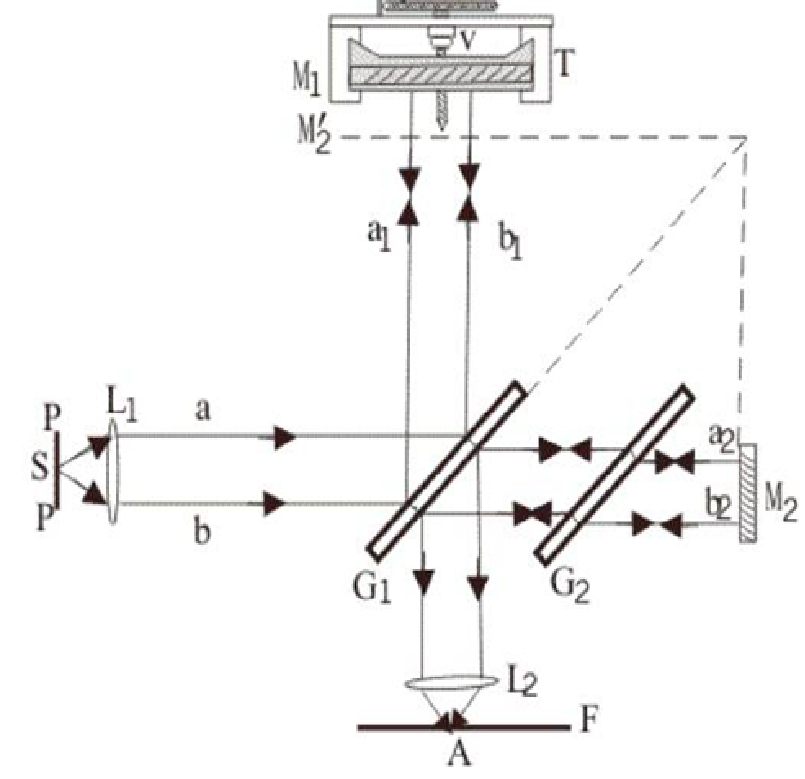
\includegraphics[width=0.8\linewidth]{picture/setup.png}
    \caption{迈克尔逊干涉实验光路原理图}
    \label{fig:setup}
\end{figure}

当迈克尔逊干涉仪的动镜 $M_2$ 与定镜 $M_1$ 的虚像 $M_1'$ 相互平行时，形成空气膜厚度为 $d$ 的等倾干涉。在透镜（或人眼）焦平面上，干涉条纹为同心圆环。对于单色光源（波长 $\lambda$），观测屏上半径为 $r$ 处的光强 $I(r)$ 可由干涉公式给出：
\begin{equation}
    I(r) = I_0 \left[ 1 + \gamma \cos(\Delta \varphi) \right]
\end{equation}
其中 $I_0$ 为背景光强，$\gamma$ 为条纹对比度。相位差 $\Delta \varphi$ 取决于光程差 $\delta$：
\begin{equation}
    \delta = 2d \cos \theta
\end{equation}
其中 $\theta$ 为折射角。在傍轴近似条件下（$\theta$ 极小），有 $\cos \theta \approx 1 - \theta^2 / 2$。若成像透镜焦距为 $f$，则 $\theta \approx r/f$。代入得：
\begin{equation}
    \delta \approx 2d \left( 1 - \frac{r^2}{2f^2} \right) = 2d - \frac{d}{f^2} r^2
\end{equation}
相位差表达式为：
\begin{equation}
    \Delta \varphi(r) = \frac{2\pi}{\lambda} \delta = \frac{4\pi d}{\lambda} - \frac{2\pi d}{\lambda f^2} r^2
\end{equation}
令中心相位 $\varphi_0 = \frac{4\pi d}{\lambda}$，空间频率系数 $k = \frac{2\pi d}{\lambda f^2}$，则：
\begin{equation}
    \Delta \varphi(r) = \varphi_0 - k r^2
    \label{eq:phase_r}
\end{equation}
由公式 (\ref{eq:phase_r}) 可见，相位 $\Delta \varphi$ 与半径 $r$ 呈二次方关系。这意味着随着半径 $r$ 增大，条纹变得越来越密（空间频率线性增加），这种非平稳信号（Chirp Signal）难以直接通过固定窗口的傅里叶变换提取单一频率。

\begin{figure}[htbp]
    \centering
    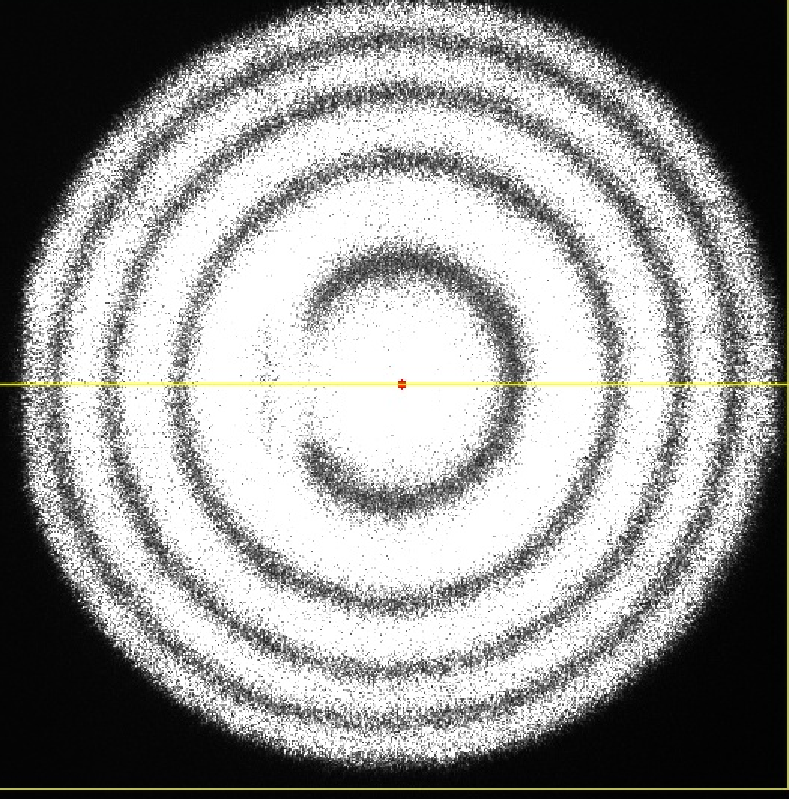
\includegraphics[width=0.45\linewidth]{picture/fringe_raw.png}
    \caption{实验采集的原始等倾干涉图样（$512 \times 512$ 像素）}
    \label{fig:raw_fringe}
\end{figure}

\subsection{变量代换与信号线性化 ($r^2$ Resampling)}
为了将非平稳信号转化为平稳信号（单频正弦波），我们引入变量代换：
\begin{equation}
    u = r^2
\end{equation}
将光强分布 $I$ 视为 $u$ 的函数 $I(u)$，则相位项变为：
\begin{equation}
    \Delta \varphi(u) = \varphi_0 - k u
\end{equation}
此时，相位 $\Delta \varphi$ 关于新变量 $u$ 呈严格线性关系。光强分布变为：
\begin{equation}
    I(u) \propto \cos(\varphi_0 - k u)
\end{equation}
这表示在 $u$ 域中，干涉图样变成了一个频率为 $k/2\pi$ 的标准余弦信号。

\subsection{算法实现流程}
基于上述物理模型，本文提出一种融合“整数级基准”与“亚波长追踪”的双模测量架构。为保证信号提取的鲁棒性，两种计数方法共享同一套基于物理模型的预处理流程。

\paragraph{1. 极坐标展开 (Polar Unwrapping)}
由于等倾干涉图样呈同心圆环分布，直接在笛卡尔坐标系下处理不仅计算复杂，且难以利用一维信号处理工具。系统首先利用 \texttt{cv.warpPolar} 将图像 $I(x,y)$ 变换为极坐标图像 $I_p(r, \theta)$。为了提高信噪比，沿角度 $\theta$ 方向取中值（或均值），得到一维径向光强分布 $S(r)$。此步骤将二维图像噪声在角度维度上进行了有效平均，显著提升了后续处理的稳定性（如图 \ref{fig:profile_r} 所示）。

\begin{figure}[htbp]
    \centering
    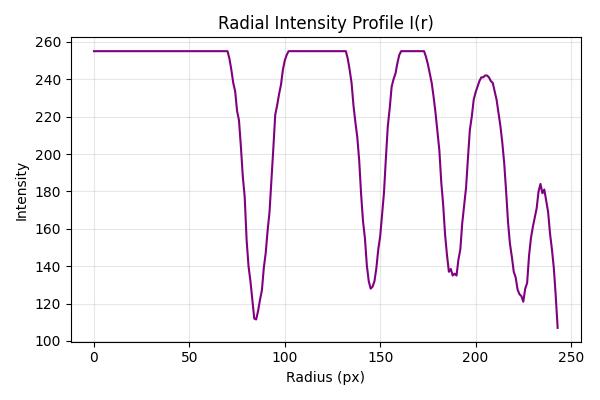
\includegraphics[width=0.7\linewidth]{picture/profile_r.png}
    \caption{极坐标展开后的径向光强分布 $I(r)$}
    \label{fig:profile_r}
\end{figure}

\paragraph{2. 非线性重采样 (Non-linear Resampling)}
为了实现 $u=r^2$ 变换，我们构造均匀分布的 $u$ 序列：$u_{lin} = \{0, \Delta u, 2\Delta u, \dots, u_{max}\}$，对应的采样半径为 $r_{sample} = \sqrt{u_{lin}}$。利用线性插值将 $S(r)$ 映射为 $S(u)$：
\begin{equation}
    S(u)[i] = S(r)\Big|_{r=\sqrt{u_i}}
\end{equation}
经过此步骤，原本随半径增大而频率非线性增加的 Chirp 信号，被映射为 $u$ 域内的单一频率正弦信号，满足了平稳信号处理的要求。

\begin{figure}[htbp]
    \centering
    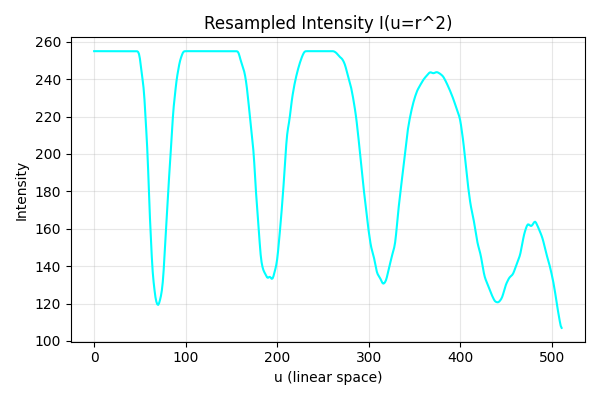
\includegraphics[width=0.7\linewidth]{picture/profile_u.png}
    \caption{重采样后的线性空间信号 $I(u)$，可见波峰处明显的饱和平台}
    \label{fig:profile_u}
\end{figure}

在完成上述统一预处理后，系统并行执行以下两种计数算法：

\subsubsection{整数级基准：光强饱和时长计数法}
在典型的迈克尔逊干涉实验中，中心视场的干涉条纹呈现“亮-暗”交替变化。尽管理论上的干涉光强遵循正弦分布，但在实际测量中，He-Ne 激光的高亮度往往导致工业相机在亮纹中心产生像素饱和（Saturation），使得波峰时域信号呈现明显的“平顶”特征（如图 \ref{fig:profile_u} 所示）。

本系统利用这一物理饱和特性，设计了极具鲁棒性的“饱和时长计数法”作为主计数手段。该方法监测重采样后圆心处（即 $u=0$ 附近）的光强信号 $I(u=0, t)$，并将其转化为二值逻辑信号：
\begin{equation}
    S(t) = \begin{cases}
        1, & \text{if } I(0,t) > I_{th} \\
        0, & \text{else}
    \end{cases}
\end{equation}
其中阈值设定为 $I_{th} = 240$（8-bit, [0, 255]）。为了彻底消除由于高频电子噪声或光强闪烁导致的误触发，算法引入了“饱和时长”判据 $t_{min}$（实验设定为 180ms）。只有当逻辑高电平 $S=1$ 的持续时间 $\Delta t > t_{min}$ 时，计数器才判定一个有效波峰通过。

这种基于二值逻辑的计数方法具有极高的抗干扰能力。它将复杂的图像分析简化为类似于数字电路中“施密特触发器”的逻辑判断，从根本上消除了光照不均、条纹畸变对整数计数的影响。只要干涉条纹对比度足以产生饱和，该方法就能提供理论上零误差的整数级波长测量基准（精度 $\lambda/2$），为后续的精密相位细分提供了可靠的绝对坐标。

\subsubsection{亚波长精度：相位追踪计数法}
在确保整数级计数准确无误的前提下，为了进一步获取 $\lambda/100$ 甚至更高的测量精度，系统采用基于频域分析的相位追踪算法（Phase Tracking）。该算法接续预处理后的 $S(u)$ 信号，包含以下步骤：

\paragraph{1. 信号增强与导数变换}
为了进一步提升在非理想光照下的特征显著性，对 $S(u)$ 施加高斯平滑并计算一阶导数 $S_{grad} = \nabla (S(u) * G_\sigma)$。这一微分操作具有双重物理意义：
\begin{itemize}
    \item \textbf{消除直流背景}：去除了照明不均产生的加性背景光 $I_{dc}$。
    \item \textbf{增强位置特征}：将原信号中平坦的饱和波峰（Intensity=255）转化为具有最大斜率的过零点（Zero-crossing），从信息论角度最大化了相位信息的费雪信息量，显著提升了相位追踪的可辨识度。
\end{itemize}

\begin{figure}[htbp]
    \centering
    \begin{subfigure}{0.48\linewidth}
        \centering
        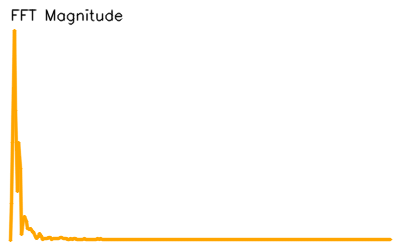
\includegraphics[width=\linewidth]{picture/fft_full.png}
        \caption{FFT 幅度谱}
    \end{subfigure}
    \hfill
    \begin{subfigure}{0.48\linewidth}
        \centering
        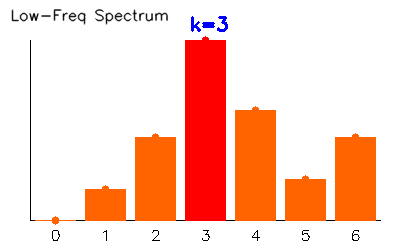
\includegraphics[width=\linewidth]{picture/fft_zoom.png}
        \caption{低频区主峰}
    \end{subfigure}
    \caption{信号频谱特征：主峰 $k$ 值（本例中 $k=3$）直接反映了视场内的条纹级数}
    \label{fig:fft}
\end{figure}

\paragraph{2. 加速归一化互相关 (FFT-NCC) 原理}
为了在 160 FPS 高帧率下精确追踪条纹位移，本系统采用频域加速的互相关算法。设参考帧 $f(n)$ 与目标帧 $g(n)$ 满足理想平移模型 $g(n) = f(n-\Delta)$。
首先根据互相关定理，时域互相关等价于频域的共轭乘积。互功率谱 $\mathcal{S}_{fg}(k)$ 为：
\begin{equation}
    \mathcal{S}_{fg}(k) = F^*(k) G(k)
\end{equation}
利用傅里叶变换的位移性质 $\mathcal{F}\{f(n-\Delta)\} = F(k)e^{-j\frac{2\pi}{N}k\Delta}$，代入上式可得：
\begin{equation}
    \mathcal{S}_{fg}(k) = F^*(k) \cdot F(k) e^{-j\frac{2\pi}{N}k\Delta} = |F(k)|^2 e^{-j\frac{2\pi}{N}k\Delta}
\end{equation}
对其进行逆变换 (IFFT)，根据维纳-辛钦定理（Wiener-Khinchin Theorem），自相关函数 $R_{ff}$ 的傅里叶变换即为功率谱 $|F(k)|^2$，因此：
\begin{equation}
    R_{raw}[m] = \text{IFFT}\{|F(k)|^2 e^{-j\frac{2\pi}{N}k\Delta}\}[m] = R_{ff}[m-\Delta]
\end{equation}
上述推导在数学上严格证明了：互相关结果本质上是自相关函数在时域上的平移，其峰值位置 $m=\Delta$ 精确对应物理位移。
为了获得归一化的相关系数 $\rho$，利用柯西-施瓦茨不等式并结合短时能量平稳假设（$\sum g^2 \approx \sum f^2$）：
\begin{equation}
    \rho[m] \approx \frac{\text{IFFT}\{F^*(k)G(k)\}[m]}{\sum |f(n)|^2}
\end{equation}
通过查找 $\rho[m]$ 的主峰位置并结合局部抛物线插值，该算法可在极低计算负荷下实现优于 0.01 像素的位移分辨率。

\begin{figure}[htbp]
    \centering
    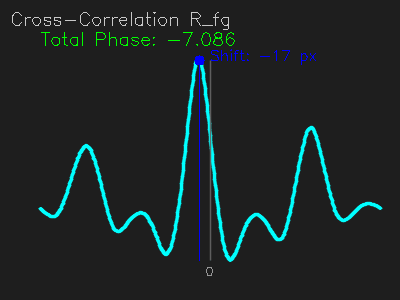
\includegraphics[width=0.7\linewidth]{picture/ncc_peak.png}
    \caption{归一化互相关 (NCC) 函数的亚像素峰值}
    \label{fig:ncc}
\end{figure}

\paragraph{3. 卡尔曼滤波相位锁定}
为了进一步应对环境微振动，系统构建了基于“均速模型”（Constant Velocity Model）的卡尔曼滤波器。利用物理位移台的大惯性特征，滤波器以预测的恒定速度推演下一时刻的相位，并将 FFT 计算的瞬时相位差作为观测值。该算法通过“预测-校正”闭环，实现了对环境高频噪声的强阻尼平滑，稳定锁定了条纹移动的亚像素轨迹。

\section{实验系统与软件架构}

\subsection{硬件架构}
本实验系统主要包括光学干涉模块与自动化控制模块，整体硬件布局如图 \ref{fig:hardware} 所示。

\begin{figure}[htbp]
    \centering
    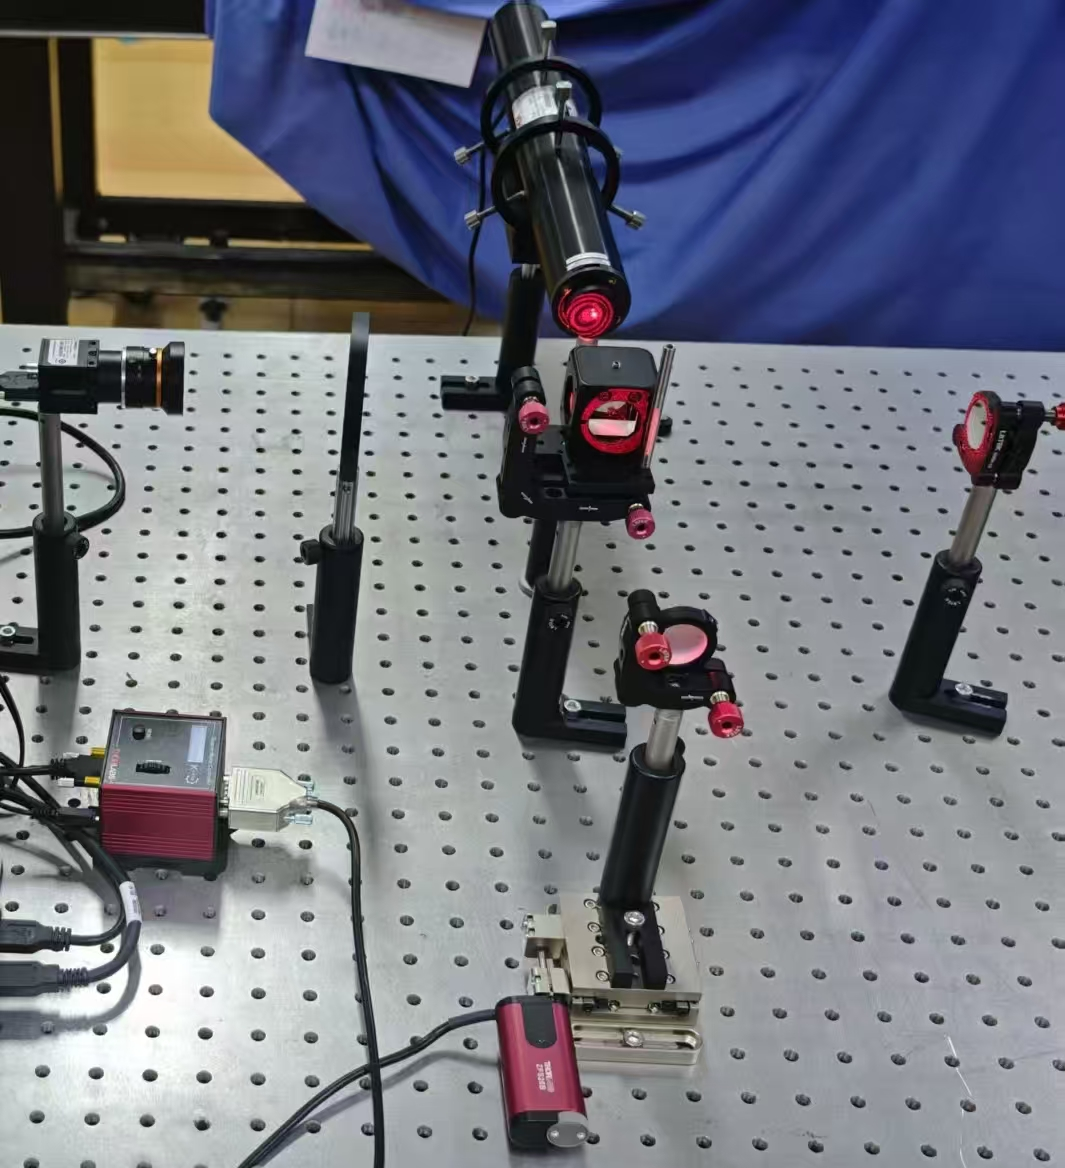
\includegraphics[width=0.8\linewidth]{picture/devices.png}
    \caption{实验装置实物图：包含激光器、干涉仪、高速相机与电动位移台}
    \label{fig:hardware}
\end{figure}

\begin{figure}[htbp]
    \centering
    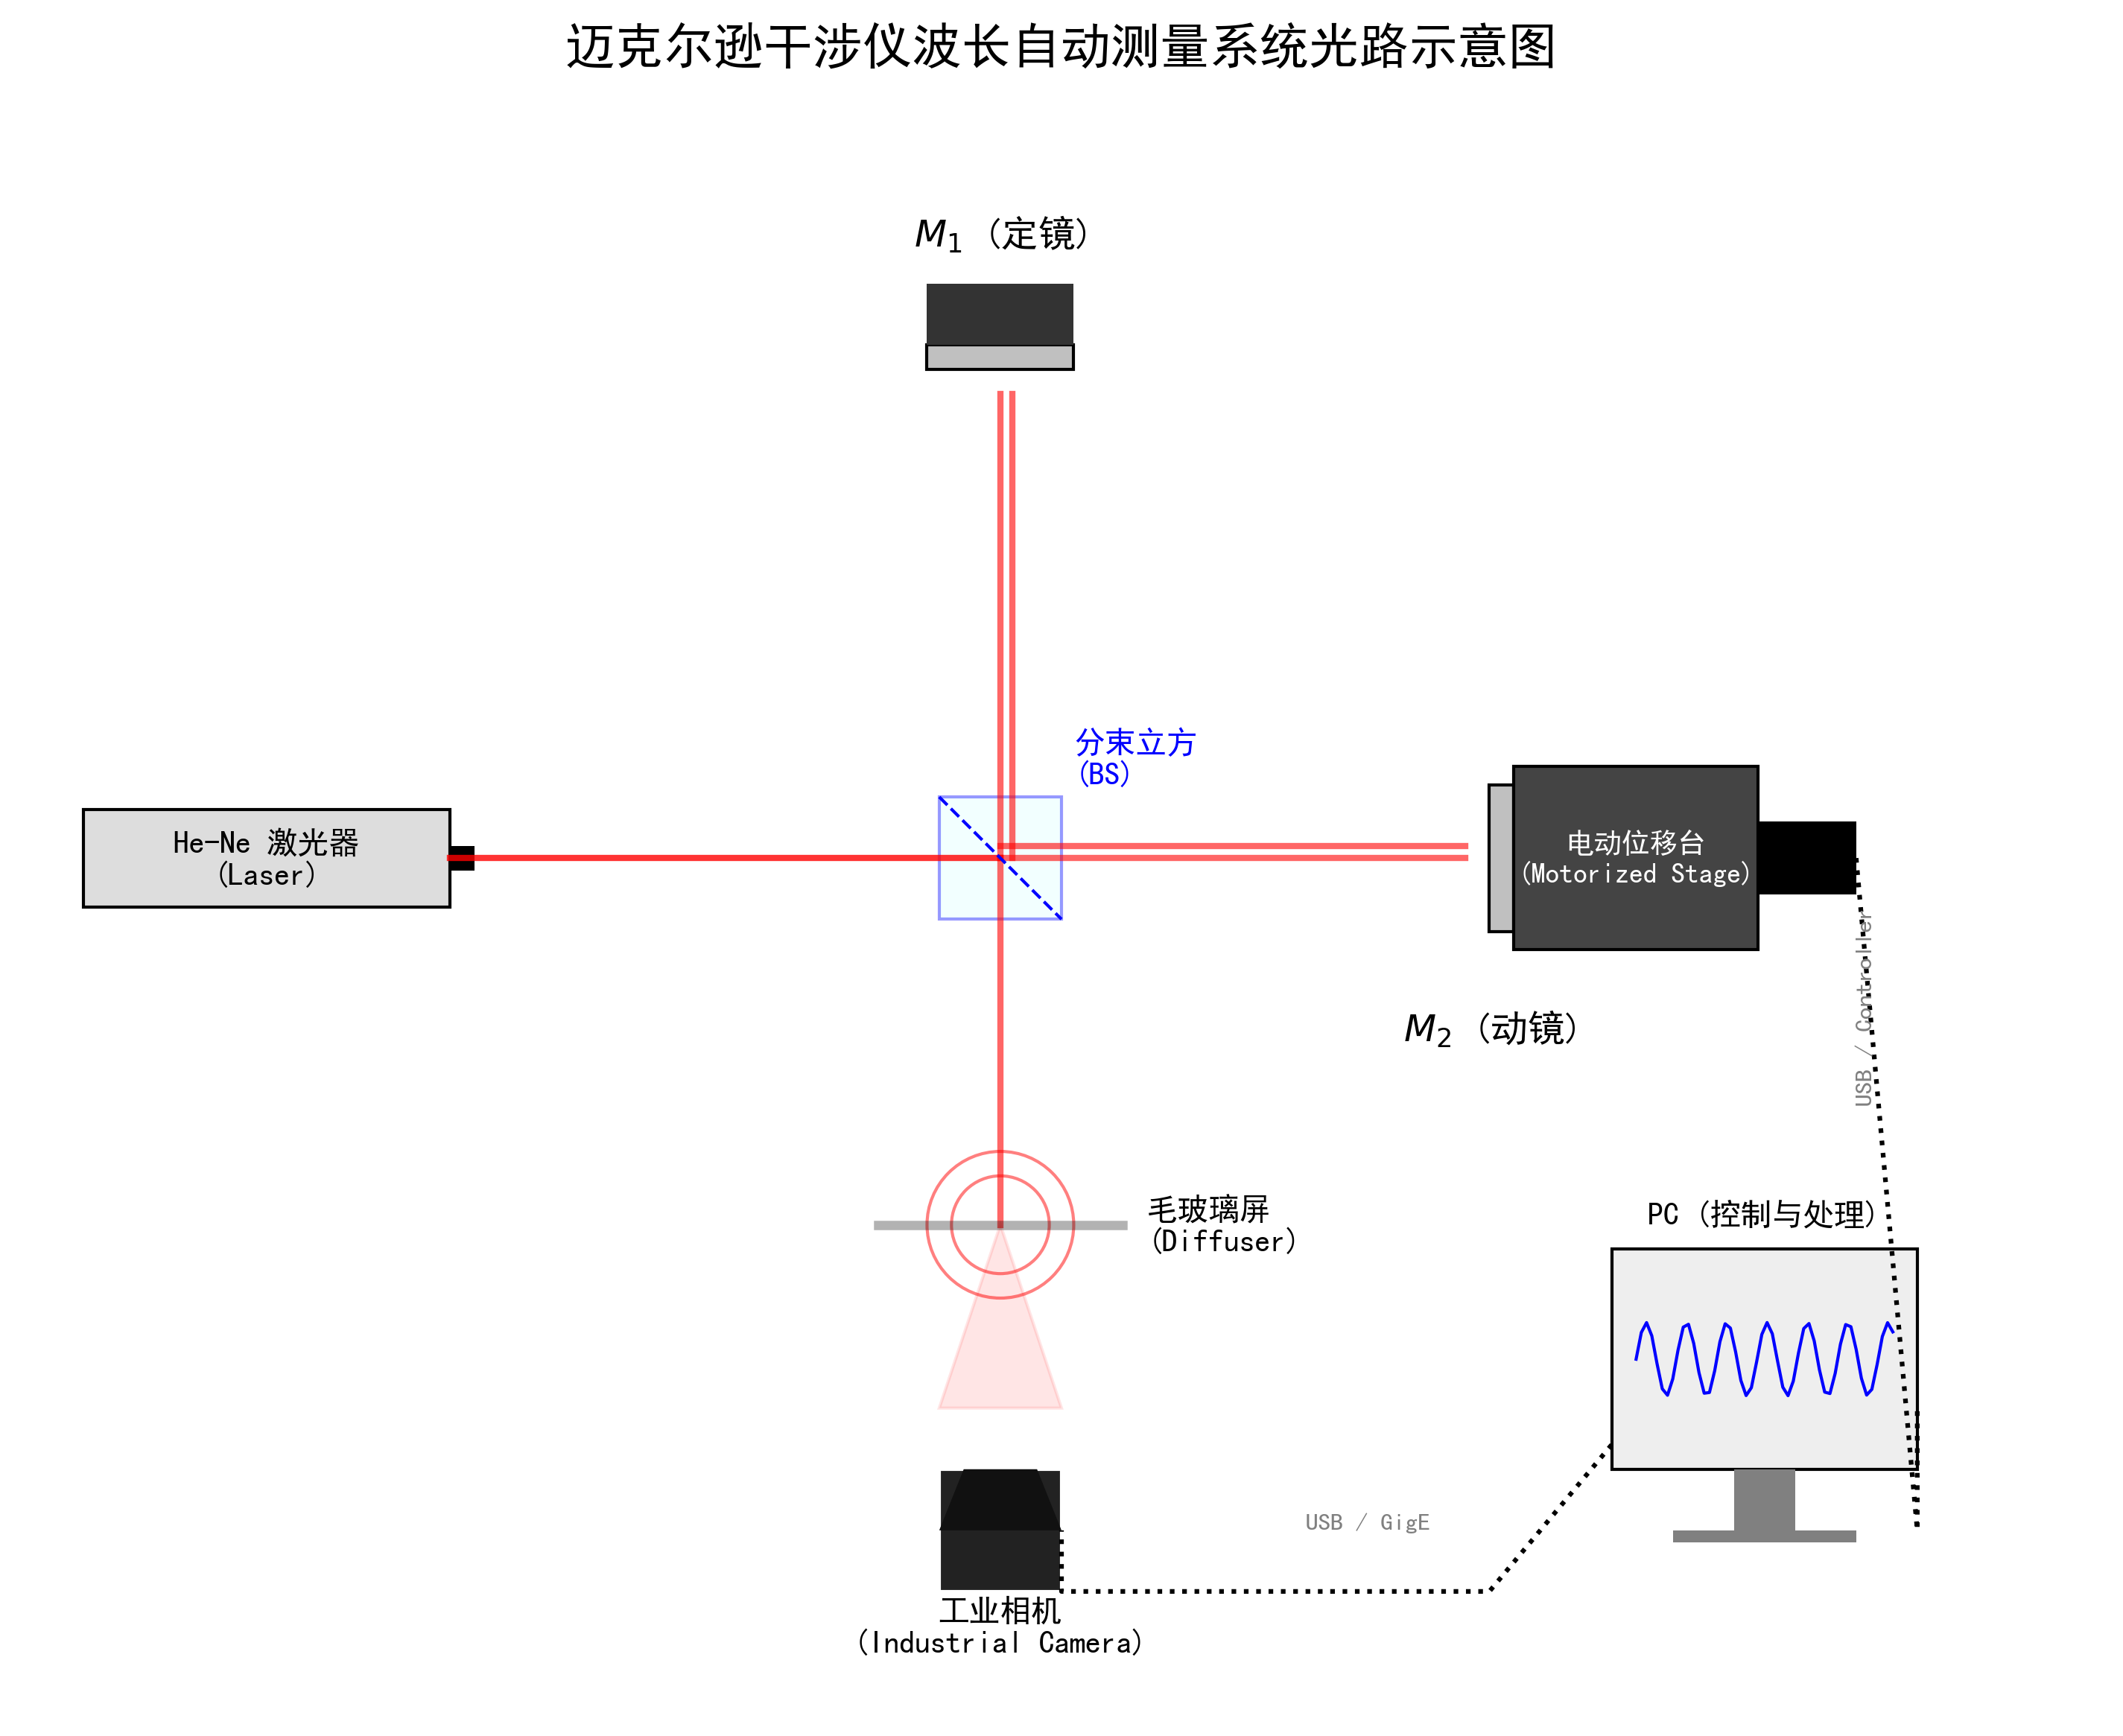
\includegraphics[width=0.75\linewidth]{picture/optical_setup_diagram.png}
    \caption{迈克尔逊干涉光路示意图}
    \label{fig:optical_path}
\end{figure}

系统光路（图 \ref{fig:optical_path}）采用经典的迈克尔逊干涉结构。光源部分选用 He-Ne 激光器 ($\lambda \approx 632.8nm$) 作为标准参考，另备有低压钠灯用于双线波长差测量。光束经分光棱镜 (BS) 分为两路，分别被定镜 $M_1$ 与动镜 $M_2$ 反射后汇聚干涉。

成像与传感部分，采用 Hikrobot MV-CA013-20GM 工业相机采集干涉圆环，最高帧率可达 160 FPS，确保了对快速移动条纹的实时捕捉。动镜 $M_2$ 由 Thorlabs Kinesis MTS50-Z8 电动位移台驱动，具备 29nm 的理论分辨率与优异的直线度，为精密波长测量提供了硬件保障。

\subsection{软件架构}
系统软件基于 Python 语言开发，采用模块化设计以保证扩展性。
\begin{itemize}
    \item \textbf{图像处理层}：基于 OpenCV 与 NumPy 实现图像的极坐标变换、高斯滤波与 FFT 运算；
    \item \textbf{硬件控制层}：通过 Thorlabs Kinesis .NET API 封装实现对位移台的 PID 闭环控制，利用 MVS SDK 实现工业相机的高速流式采集；
    \item \textbf{交互界面层}：利用 Tkinter 构建多线程 GUI，分离 UI 渲染与后台算法，避免界面卡顿。
\end{itemize}

\subsection{集成控制台}
为了简化操作流程，本系统开发了可视化的集成控制台（如图 \ref{fig:console} 所示）。

\begin{figure}[htbp]
    \centering
    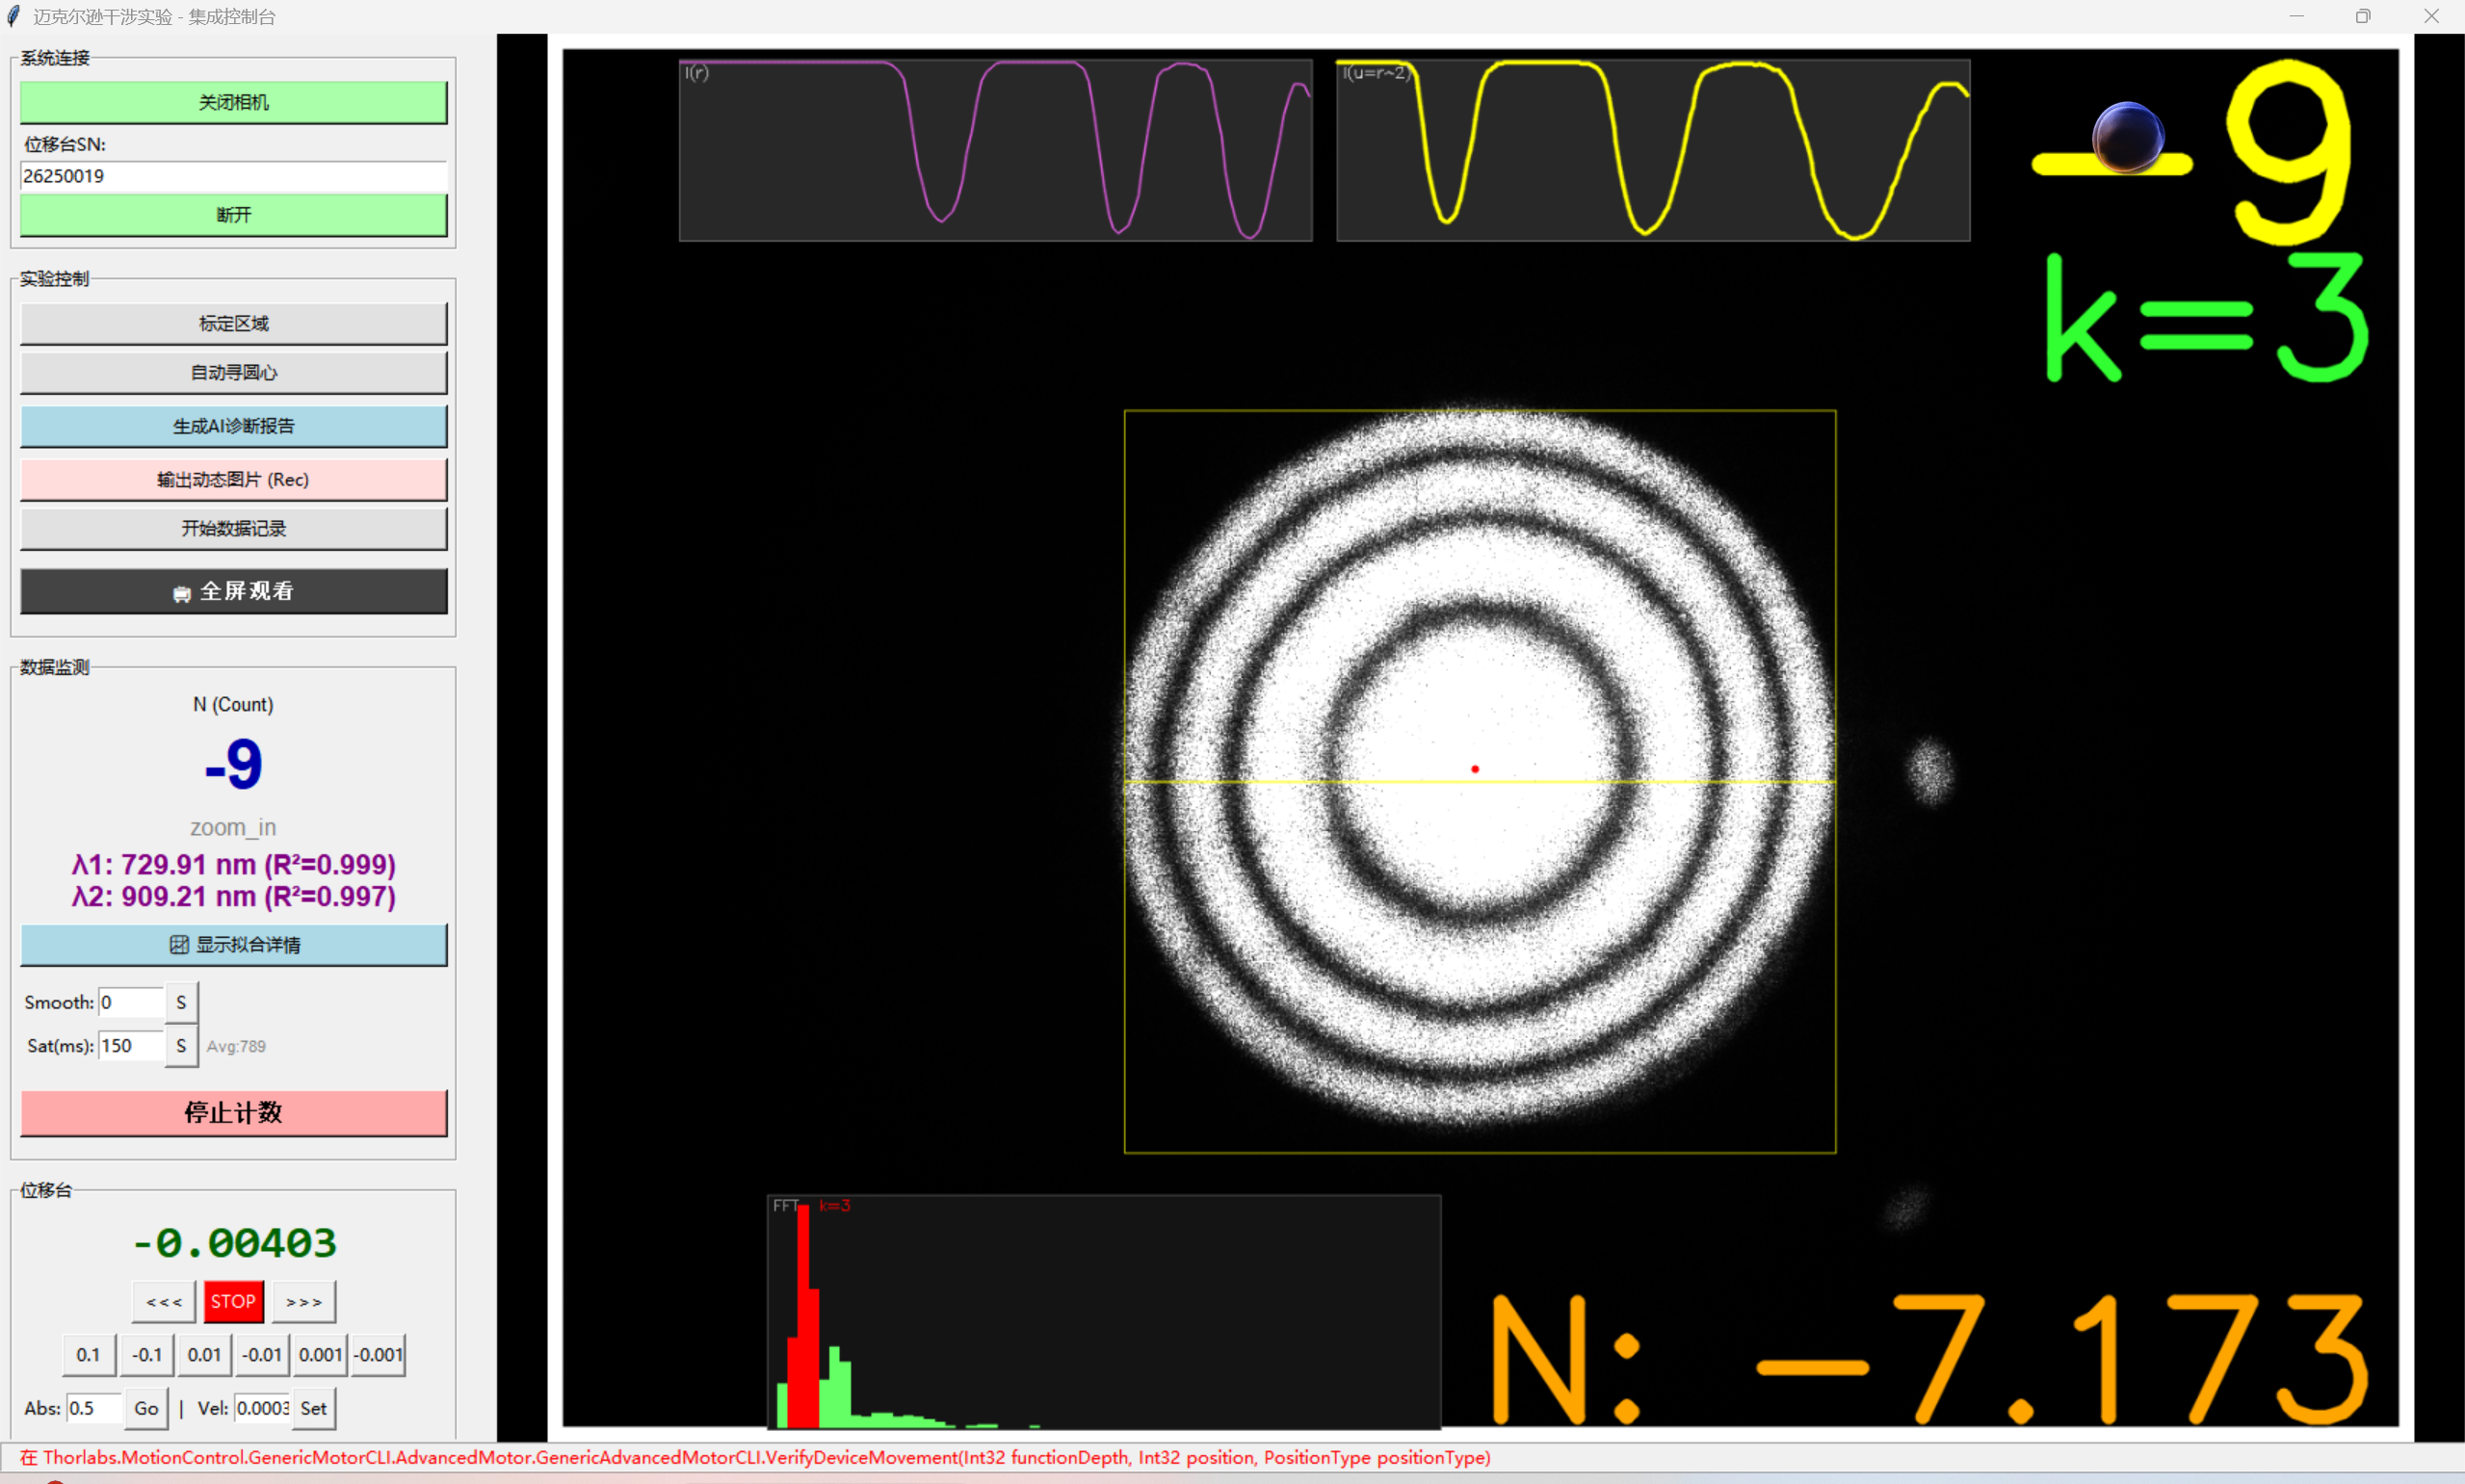
\includegraphics[width=1.0\linewidth]{picture/controller.png}
    \caption{系统集成控制台用户界面}
    \label{fig:console}
\end{figure}

控制台集成了实时视频预览、波长计算面板、位移台运动控制与波形诊断功能。用户可通过“Setup Mode”一键划定感兴趣区域 (ROI)，软件自动锁定干涉圆心。界面实时显示相位吞吐量 $N$、实时位移 $d$ 及拟合波长 $\lambda$，并支持以 CSV 格式导出带有时间戳的完整实验数据，极大提升了实验效率。

\section{实验过程}
\subsection{系统初始化与标定}
系统启动后，首先进行光路粗调，使背景光斑均匀且对比度良好。随后在软件界面进入“Setup Mode”，手动划定感兴趣区域（ROI）及大概圆心。此步骤可消除算法在初始阶段因圆心搜索波动带来的误差。

\subsection{回程误差补偿 (Backlash Compensation)}
由于机械丝杆传动系统存在公差，当电机换向或初始启动时，往往存在位移台丝杆转动但台面未产生有效位移的“死区”（Backlash）。在此期间，编码器读数发生变化，但干涉条纹静止，若直接计入会导致波长计算偏大（斜率偏小）。

本系统设计了动态监测逻辑：在每次拟合开始的初始阶段（如前 $1 \mu m$ 行程），实时监测相位变化率 $m_{local} = \Delta \Phi / \Delta d$。只有当 $m_{local}$ 超过预设阈值时，系统才判定位移台已“咬合”并开始有效记录数据，否则自动复位数据缓冲区。

\subsection{对测量数据的采集}
设定从起始位置 $d_{start}$ 移动至 $d_{end}$。上位机记录每一时刻的：
\begin{itemize}
    \item 位移台位置读数 $P(t)$ (mm)
    \item 累积相位吞吐量 $N(t) = \frac{\Phi_{total}(t)}{2\pi}$
    \item 条纹视见度（Visibility）
\end{itemize}
支持在不同速度下（$0.0001 - 0.01 mm/s$）进行多次重复测量。

\section{数据处理与不确定度评定}
\subsection{线性回归模型}
对于迈克尔逊干涉实验，累积干涉条纹数 $N$ 与动镜位移 $d$ 之间满足严格的线性关系。考虑空气折射率 $n_{air}$ 的影响，光程差变化 $\Delta \delta = 2 n_{air} \Delta d = \lambda_{vac} \Delta N$。因此，真空波长 $\lambda_{vac}$ 可表示为：
\begin{equation}
    \lambda_{vac} = 2 n_{air} \cdot \left( \frac{\Delta d}{\Delta N} \right) = \frac{2 n_{air}}{k_{fit}}
\end{equation}
其中 $k_{fit}$ 为 $N-d$ 数据的线性拟合斜率。

\subsection{测量不确定度来源分析}
本实验的不确定度主要由以下两类分量构成：

\subsubsection{A 类不确定度（统计误差）}
源于环境微振动、空气最大折射率涨落及相机读数噪声。通过最小二乘法（Ordinary Least Squares, OLS）对 $M$ 组数据点 $(d_i, N_i)$ 进行拟合，斜率 $k_{fit}$ 的标准不确定度 $u(k_{fit})$ 可由残差平方和（SSR）估计：
\begin{equation}
    u(k_{fit}) = \sqrt{\frac{\sum (N_i - \hat{N}_i)^2}{(M-2) \sum (d_i - \bar{d})^2}}
\end{equation}
在典型实验条件（移动距离 $2\text{mm}$，采样点数 $>1000$）下，高精度的 FFT-NCC 算法使线性相关系数 $R^2 > 0.9999$，A 类相对不确定度通常小于 $10^{-4}$。

\subsubsection{B 类不确定度（系统误差）}
\begin{enumerate}
    \item \textbf{位移台定位误差 $u(d)$}：实验采用 Thorlabs Kinesis KDC101 控制的 MTS50-Z8 电动位移台（或同等精度型号），其典型单向重复定位精度为 $1.5 \mu m$，全量程线性度误差约为 $0.05\%$。
    \item \textbf{余弦误差 $u(\theta)$}：若激光入射光轴与导轨移动轴存在微小夹角 $\alpha$，测量值 $\lambda_{meas} = \lambda_{true} / \cos \alpha \approx \lambda_{true} (1 + \alpha^2/2)$。经仔细调节，可控制 $\alpha < 0.5^\circ$，由此引入的相对误差约为 $3.8 \times 10^{-5}$。
    \item \textbf{空气折射率 $u(n)$}：标准空气折射率 $n_0 \approx 1.00027$。由 Edlén 公式可知，温度变化 $1^\circ \text{C}$ 或气压变化 $0.4\text{kPa}$ 引入的修正量约为 $10^{-6}$ 量级，可忽略不计。
\end{enumerate}

\subsection{合成不确定度}
波长测量的合成相对标准不确定度 $u_r(\lambda)$ 为：
\begin{equation}
    u_r(\lambda) = \sqrt{ \left( \frac{u(k_{fit})}{k_{fit}} \right)^2 + u_{sys}^2 }
\end{equation}
综合考虑，系统总测量不确定度主要受限于导轨直线度与光路准直性，预期精度可达 $0.1\% \sim 0.05\%$。

\section{应用与展望}
\subsection{钠光双线波长差测量}
本系统扩展支持钠光实验。由于钠黄光包含 $\lambda_1 = 589.0 nm$ 和 $\lambda_2 = 589.6 nm$ 两条谱线，随光程差增加，两者条纹发生“相长-相消”的拍频现象。
系统实时记录视见度（Visibility）曲线，通过分析视见度包络的极小值间距 $\Delta d_{beat}$，可自动反演波长差：
\begin{equation}
    \Delta \lambda = \frac{\lambda_{avg}^2}{2 \Delta d_{beat}}
\end{equation}

\subsection{机器智能辅助}
当前系统已集成基础的 AI 报告生成功能。未来展望引入深度卷积神经网络（CNN）直接对极低对比度的干涉图样进行端到端相位预测，以进一步提升在复杂环境光下的测量稳定性。

\appendix
\section{附录：核心算法数理基础详述}

\subsection{离散信号的频域处理基础}
为了从有限长度的离散采样信号中提取高精度的相位信息，必须有效处理频谱泄漏（Spectral Leakage）与直流分量（DC Component）干扰。
\begin{itemize}
    \item \textbf{汉宁窗 (Hanning Window) 抑制泄漏}:
          由于干涉条纹并不是严格周期的，且采样窗口长度往往不是信号周期的整数倍，直接截断会导致频谱能量泄露到旁瓣。系统在 FFT 变换前施加汉宁窗 $w(n) = 0.5 - 0.5\cos(2\pi n / (N-1))$。该窗函数通过平滑边界将信号两端强制归零，其旁瓣衰减达 -31dB（相比矩形窗的 -13dB），有效抑制了非周期截断带来的高频伪影，显著提高了主频峰值的信噪比。

    \item \textbf{梯度滤波器 (Gradient High-pass Filter)}:
          背景光强往往存在低频不均匀分布（Vignetting）。数值一阶差分算子 $h = [-1, 0, 1]$ 的频率响应为 $H(\omega) = i \sin(\omega)$。在零频处 $\omega \to 0$，响应 $|H(\omega)| \to 0$，从而完全阻断了背景直流分量 $I_{dc}$。对于理想干涉信号 $I(u) = I_{dc} + A \cos(\omega u + \phi)$，经梯度变换后变为 $I'(u) \approx -A\omega \sin(\omega u + \phi)$。此操作不仅去除了光照不均，还将原本在饱和区（Intensity=255）平坦的波峰转化为具有最大斜率的过零点（Zero-crossing），从信息论角度最大化了位置信息的费雪信息量（Fisher Information）。
\end{itemize}



\subsection{亚像素峰值估计的几何演变推导}
FFT-NCC 的整数步进限制了位移的分辨率。为实现纳米级位移探测，系统利用相关函数峰值附近的局部抛物线特征进行亚像素提取。

\subsubsection{1. 局部二阶泰勒建模}
假设相关函数 $\rho(x)$ 在真实峰值 $x_{true}$ 处（相对整数峰值 $x_0$ 偏移为 $\delta$）满足二阶可微。对其进行展开：
\begin{equation}
    y(x) = a(x - \delta)^2 + c
\end{equation}
其中 $\delta$ 为待求偏移，$a$ 为曲率，$c$ 为峰值。

\subsubsection{2. 方程组解析计算}
选取以 $x_0$ 为中心的三个邻域采样点 $(-1, y_{-1})$, $(0, y_0)$, $(1, y_{+1})$，可建立方程组：
\begin{align}
    y_{-1}   & = a(-1 - \delta)^2 + c = a(1 + 2\delta + \delta^2) + c \\
    y_{0} \  & = a\delta^2 + c                                        \\
    y_{+1}   & = a(1 - \delta)^2 + c = a(1 - 2\delta + \delta^2) + c
\end{align}
计算一阶中心差分：
\begin{equation}
    y_{-1} - y_{+1} = 4a\delta \implies \delta = \frac{y_{-1} - y_{+1}}{4a}
    \label{eq:delta_step1}
\end{equation}
进一步利用二阶中心差分算子提取曲率 $a$：
\begin{align}
    (y_{-1} - y_0) + (y_{+1} - y_0) & = y_{-1} + y_{+1} - 2y_0 \nonumber                 \\
                                    & = 2a \implies a = \frac{y_{-1} - 2y_0 + y_{+1}}{2}
    \label{eq:a_step2}
\end{align}
将 (\ref{eq:a_step2}) 代入 (\ref{eq:delta_step1})，得最终位移估值公式：
\begin{equation}
    \delta = \frac{y_{-1} - y_{+1}}{2(y_{-1} - 2y_0 + y_{+1})}
\end{equation}
最终测得位置为 $x_{measure} = x_0 + \delta$。

\subsection{自适应扩展卡尔曼滤波 (AEKF) 的稳态分析}
本节阐述基于均速模型的状态观测器。

\subsubsection{1. 状态递归关系}
定义系统状态 $x_k$ 为位移速率，状态转移矩阵 $\mathbf{F} = [1]$。预测方程为：
\begin{equation}
    \hat{x}_k^- = \hat{x}_{k-1}, \quad P_k^- = P_{k-1} + Q
\end{equation}
其中 $Q \approx 10^{-6}$，确保系统具有极强的惯性记忆。

\subsubsection{2. 极值扰动下的增益特性}
当新息残差 $|\tilde{y}_k| > T_{gate}$ 时，观测噪声设定为 $R_{reject} \to \infty$。此时卡尔曼增益变为：
\begin{equation}
    \lim_{R_k \to \infty} K_k = \lim_{R_k \to \infty} \frac{P_k^-}{P_k^- + R_k} = 0
\end{equation}
代入后验更新公式：
\begin{equation}
    \hat{x}_k = \hat{x}_k^- + K_k \tilde{y}_k \approx \hat{x}_k^-
\end{equation}
该推导证明了滤波器在无法获取可信测量时，将自动退化为纯预测模式，利用模型惯性在扰动期间维持数值输出的连续性。

\end{document}